\documentclass[a4paper, 11pt, spanish]{article}

% ---------------- Paquetes de formato.
\usepackage[spanish]{babel} % Para codificar el texto.
\usepackage[top=70mm, bottom=30mm, left=18mm, right=18mm]{geometry} % Para modificar el tamaño de las hojas.
\usepackage{fancyhdr} % Para poner la institución, dpto y curso arriba.
\usepackage{parallel} % Para escribir en columnas (Poner los integrantes a la derecha).
\usepackage[firstpage=false]{background} % Para poner el logo de la U arriba en todas las páginas.
\usepackage{enumerate} % Para poder enumerar como a), b), etc.
\usepackage[utf8]{inputenc} % Para usar acentos en vez de \'.

% ---------------- Paquetes graficos.
\usepackage{graphicx} % remove the demo option.
\usepackage{tikz}
\usepackage{caption}
\usepackage{subcaption} % Para usar sub-figuras

% ---------------- Paquetes matematicos.
\usepackage{amsmath} % Para poder hacer N^o y se vea bonito.
\usepackage{amsthm} % Fonts matematicos.
\usepackage{amssymb} % Para usar \therefore
\usepackage{commath} % Para usar \abs y \norm

% ---------------- Paquetes 'computines'.
\usepackage{listings} % Para escribir codigo y que se vea bonito.
\usepackage[% Descomentar las opciones a usar.
spanish,
%boxed, % Encierra los algoritmos en un cuadro.
boxruled, % Encierra los algoritmos en un cuadro colocando el titulo al comienzo.
%ruled, % Coloca una linea al comienzo y otra al final del algoritmo. El titulo de este queda al comienzo del algoritmo.
%algoruled, % Lo mismo que el anterior pero mas espaciado.
%tworuled, % Como ruled pero sin una linea al comienzo.
%algochapter, % Los algoritmos se enumeran segun capitulo.
%algopart, % Los algoritmos se enumeran por partes.
%figure, % Los algoritmos son considerados figuras (y por ende salen en \listoffigures).
%linesnumbered, % Enumera las lineas.
longend % Los end son para cada ciclo, por ejemplo endif para los if-else.
]{algorithm2e}

% ---------------- Paquetes miscelaneos.
%\usepackage{lipsum} % Para hacer placeholders.
\usepackage{bohr} % Para dibujar atomos.

% ---------------- Comando mas corto para insertar figuras. Ojo que deben estar guardadas en ./img/
% \fig{name}{width}{height}{caption}
\newcommand{\fig}[4]{%
	\begin{figure}[!htbp]
		\centering
		\includegraphics[width=#2, height=#3]{img/#1}
		\caption{#4}
	\end{figure}
}
% ejemplo:
%			\fig{nombre_imagen.png}{10cm}{5cm}{Titulo de la imagen}


%\begin{figure}[!ht]
%\centering
%\begin{subfigure}{.5\textwidth}
%  \centering
%  \includegraphics[width=10cm, height=8cm]{img/curva0f1.pdf}
%  \caption{Curva de nivel 0 de $F_{1}$.}
%  \label{fig:sub1}
%\end{subfigure}%
%\begin{subfigure}{.5\textwidth}
%  \centering
%  \includegraphics[width=10cm, height=8cm]{img/curva0f2.pdf}
%  \caption{Curva de nivel 0 de $F_{2}$.}
%  \label{fig:sub2}
%\end{subfigure}
%\caption{Curvas de nivel 0 de $F_{1}$ y $F_{2}$}
%\label{fig:test}
%\end{figure}


% ---------------- Comando para hacer itemes
% \Solution{pregunta}{solucion}
\newcommand{\Solution}[2]{%
	\item #1 \vspace{0.2cm}
	\textbf{Soluci\'on:} #2
}
% \Demonstration{pregunta}{demostracion}
\newcommand{\Demonstration}[2]{%
	\item #1 \vspace{0.2cm}
	\begin{proof}
		#2	
	\end{proof}
}

% ---------------- Opciones de algortihm2e
\SetKw{KwRequire}{Require:}

% ---------------- Opciones de background.
\SetBgColor{black}
\SetBgScale{1}
\SetBgOpacity{1}
\SetBgAngle{0}
\SetBgContents{%
	\begin{tikzpicture}[remember picture,overlay]
		\node at (-8.0,0.746\textheight) {
\includegraphics[height=18mm,width= 0.155\textwidth]{img/LogoUIngenieria.png}};
	\end{tikzpicture}
}

% ---------------- Creacion de institucion, departamento y curso.
\fancyheadoffset[L]{-2cm}
\fancyhead[L]{\footnotesize{\textbf{\textsf{Universidad de Chile \\ Facultad de Cs. F\'isicas y Matem\'aticas \\ Departamento de F\'isica \\ FI3104-1: M\'etodos Num\'ericos para la Ciencia e Ingenier\'ia. }}}}
\renewcommand{\headrulewidth}{0pt}
\setlength{\voffset}{-3cm}

\pagestyle{fancy} % Estilo de las páginas

\begin{document}

\pagenumbering{gobble} % Quita el numero de las paginas (y las resetea a 1)

\clearpage

\thispagestyle{fancy}
\vspace*{6.5cm} % Espacio vertical para posicionar bien el título (En una de esas esto se puede optimizar para que no sea tan a la fuerza bruta).

% ---------------- Titulo.
\begin{center}
	\Large{\textbf{\textsf{Tarea $\text{N}^\text{o}$3}}} \\
	\huge{\textbf{\textsf{Interpolaci\'on de Polinomios.}}}
\end{center}

\vspace*{5.5cm}

% ---------------- Integrantes, profes, etc.
\begin{Parallel}{1cm}{7.5cm}
	\ParallelRText{%
		\begin{flushright} % Tira el texto hacia la derecha.
			\large{%
				\textsf{%
					\begin{tabular}{rl}
%						Integrantes: &
%							\begin{tabular}[t]{@{}l@{}}
%								Integrante 1. \\
%								Integrante 2.
%							\end{tabular} \\
						& Jos\'e Ignacio Vines. \\
						Profesor: & 
							\begin{tabular}[t]{@{}l@{}}
						 		Valentino Gonz\'alez.
							\end{tabular} \\
						Auxiliares: &
							\begin{tabular}[t]{@{}l@{}}
								Mario Aguilar. \\
								Ignacio Armijo. \\
								Mar\'ia Constanza Flores. \\
							\end{tabular} \\	
%						Ayudantes: &
%							\begin{tabular}[t]{@{}l@{}}
%								Ayudante 1. \\
%								Ayudante 2.
%							\end{tabular} \\		 
					\end{tabular}
					Fecha: \today
				}
			}
		\end{flushright}
	}
\end{Parallel}

\clearpage

\pagenumbering{arabic} % Numeros de pagina Arabicos (y los resetea a 1)

\newpage

\tableofcontents % Indice. Descomente para usar.
\listoffigures % Lista de figuras. Descomente para usar.
%\listoftables % Lista de tablas. Descomente para usar.

\newpage

\section{Introducci\'on}
La fotometr\'ia es el \'area de la ciencia donde se mide la luz, es decir, la cantidad de fotones que llegan a partir de una fuente. En particular, en astronom\'ia se cuantifican los fotones que llegan por estrella. Una de las razones por las que esto se estudia es para buscar exoplanetas: al tomar la luz que proviene de una estrella y medirla peri\'odicamente por un tiempo, uno forma una curva de luz: si en esa curva hay decrecimientos bruscos, puede ser porque hay un planeta orbitando que tapa peri\'odicamente la luz proveniente de la estrella. 

Hay varias t\'ecnicas de fotometr\'ia; para este trabajo, se utiliza una llamada Fotometr\'ia de Apertura. \'Esta consiste en tomar la imagen de la estrella y elegir un radio de apertura, el cual define un c\'irculo dentro del cual debiese estar todo el flujo de la estrella, para integrar el brillo proveniente de ese c\'irculo (es decir, sumar la informaci\'on de los electrones exitados en ese pixel del CCD). Con esto, se obtiene la intensidad de la luz proveniente de toda la estrella. Adem\'as del radio de apertura, se elige un anillo alrededor de la estrella (caracterizado por dos radios) el cual se usa como correcci\'on, ya que el cielo alrededor de la estrella no es completamente negro en la imagen captada.


El objetivo de este trabajo es armar desde cero las herramientas computacionales que se utilizan para hacer fotometr\'ia de apertura. Se debe armar el programa que, teniendo los datos, puedan leerlos y realizar una lectura de la cantidad de luz (cantidad de electrones exitados en la placa CCD). El programa se hace en lenguaje Python 2.7, usando el paquete astropy.io para el manejo de los archivos que se entregan (de extensi\'on .fits) y scipy para las funciones matem\'aticas necesarias.

\section{Procedimiento}
\subsection{Comparaci\'on de M\'etodos}
Para comparar como funcionan los m\'etodos, \'estos se aplicar\'an a una funci\'on Gaussiana definida como sigue:
\begin{equation}
	f(x) = e^{-x^{2}/0.05}
\end{equation}

En primera instancia se divide el intervalo $[-1,1]$ en 4 tramos equiespaciados con la funci\'on \textbf{linspace}, dejando un total de 5 puntos para llevar a cabo la interpolaci\'on, luego, haciendo uso del m\'odulo \textbf{scipy.interpolate} y de la funci\'on \textbf{lagrange} y clase \textbf{UnivariateSpline} se hace la interpolaci\'on, aumentando en 5 el n\'umero de puntos para la interpolaci\'on hasta llegar a 20, siempre manteniendo el equiespaciado del intervalo.

La funci\'on \textbf{lagrange} recibe como argumentos dos vectores, $x$ e $y = f(x)$: un vector con el intervalo de puntos a samplear, uno con la funci\'on evaluada en dichos puntos respectivamente, y retorna un polinomio de Lagrange que pasa por todos los puntos de $x$. Como nota adicional, la implementaci\'on de Spline es num\'ericamente inestable y el resultado s\'olo es confiable hasta un intervalo con veinte puntos\footnote{http://docs.scipy.org/doc/scipy/reference/generated/scipy.interpolate.lagrange.html\#scipy.interpolate.lagrange}.

La clase \textbf{UnivariateSpline} recibe como argumentos dos vectores, $x$ e $y = f(x)$: un vector con el intervalo de puntos a samplear y uno con la funci\'on evaluada en dichos puntos respectivamente, y como par\'ametros adicionales recibe $s$, un factor de suavidad utilizado para elegir el n\'umero de nudos del Spline, y $k$, el orden del Spline. Se elige $s=0$ para que pase por todos los puntos del intervalo y $k=3$ para que sea un Spline c\'ubico. Esta clase instancia un objeto de tipo \textbf{UnivariateSpline}, que representa un Spline que pasa por todos los puntos de $x$, que luego se puede evaluar.

La clase \textbf{UnivariateSpline} es un wrapper de FITPACK, un paquete de subrutinas escrito en FORTRAN utilizado para calcular Splines suaves para distintos tipos de datos y geometr\'ias\footnote{http://www.netlib.org/dierckx/}; en particular \textbf{UnivariateSpline} hace uso de la subrutina \textbf{fpcurf0}, que a su vez utiliza la subrutina \textbf{fpcurf}\footnote{El archivo fpcurf.f est\'a incluido en la carpeta for\_routines en el repositorio.} para calcular el Spline.
La condici\'on de suavidad que se debe cumplir en los nodos es que la k-\'esima derivada del Spline sea 0. La documentaci\'on de \textbf{fpcurf} no contiene informaci\'on de c\'omo maneja la implementaci\'on los extremos del intervalo, sin embargo la implementaci\'on cl\'asica del m\'etodo de Spline es imponer que la segunda derivada del Spline en los extremos sea 0, as\'i el Spline sigue una l\'inea recta desde los extremos.

\subsection{Reparaci\'on de Imagen}
Primero, usando el m\'odulo \textbf{skimage}, \textbf{skimage.io} y la funci\'on \textbf{img\_as\_float}, se carga la imagen a reparar como un tensor de floats, compuesto por tres matrices que representan las capas R, G y B (red, green y blue) de la imagen. Luego de cargar la imagen se toma una estampilla de la imagen, es decir, se toma la secci\'on de esta que requiere reconstrucci\'on. Utilizando la funci\'on \textbf{scipy.where} se eligen los puntos de la estampilla no tiene errores para la interpolaci\'on, despu\'es de obtener los puntos en donde la estampilla no tiene pixeles muertos se hace una interpolaci\'on Spline en dos dimensiones para cada capa de la estampilla utilizando la clase \textbf{SmoothBivariateSpline}, luego se arreglan los puntos da\~nados por capa y se juntan todas para recrear la imagen original reconstruida.

La clase \textbf{SmoothBivariateSpline} tambi\'en es un wrapper de FITPACK. Esta clase en particular utiliza la subrutina \textbf{surfit}. La clase recibe tres vectores de una dimensi\'on; $x, y, z$; que representan las coordenadas de los puntos para la interpolaci\'on (es necesario notar que el orden de estos argumentos no es importante para el funcionamiento del algoritmo), y un par\'ametro adicional $kx$ y $ky$, los \'ordenes del Spline para $x$ e $y$ respectivamente, \'estos se eligen como $kx = ky = 3$.

A la clase \textbf{SmoothBivariateSpline} se le dio como argumentos los bordes de la estampilla y un vector con los valores de la estampilla en todos los pixeles no da\~nados.

\section{Resultados}
La figura 1 muestra la interpolaci\'on con polinomios de Lagrange. De la figura se aprecia que \'esta aproximaci\'on es m\'as fiel a la funci\'on original a medida se aumenta la cantidad de puntos utilizados para la interpolaci\'on, sin embargo a los extremos se observa un comportamiento oscilatorio de la aproximaci\'on, conocido como el Fen\'omeno de Runge\footnote{https://en.wikipedia.org/wiki/Runge\%27s\_phenomenon}.

La figura 2 muestra la interpolaci\'on con Spline. A mayor cantidad de puntos la interpolaci\'on con Spline es mejor aproximaci\'on que la interpolaci\'on con Lagrange. La interpolaci\'on con Spline no presenta el Fen\'omeno de Runge cuando se usa una cantidad grande de puntos.

La figura 3 muestra la diferencia entre ambos m\'etodos de interpolacion y la funci\'on original. Se puede apreciar de ella que la aproximaci\'on Spline es mejor que la aproximaci\'on con Lagrange.

La figura 4 muestra la imagen de la galaxia reconstruida.
\begin{figure}[!hbpt]
\centering
\begin{subfigure}{.5\textwidth}
  \centering
  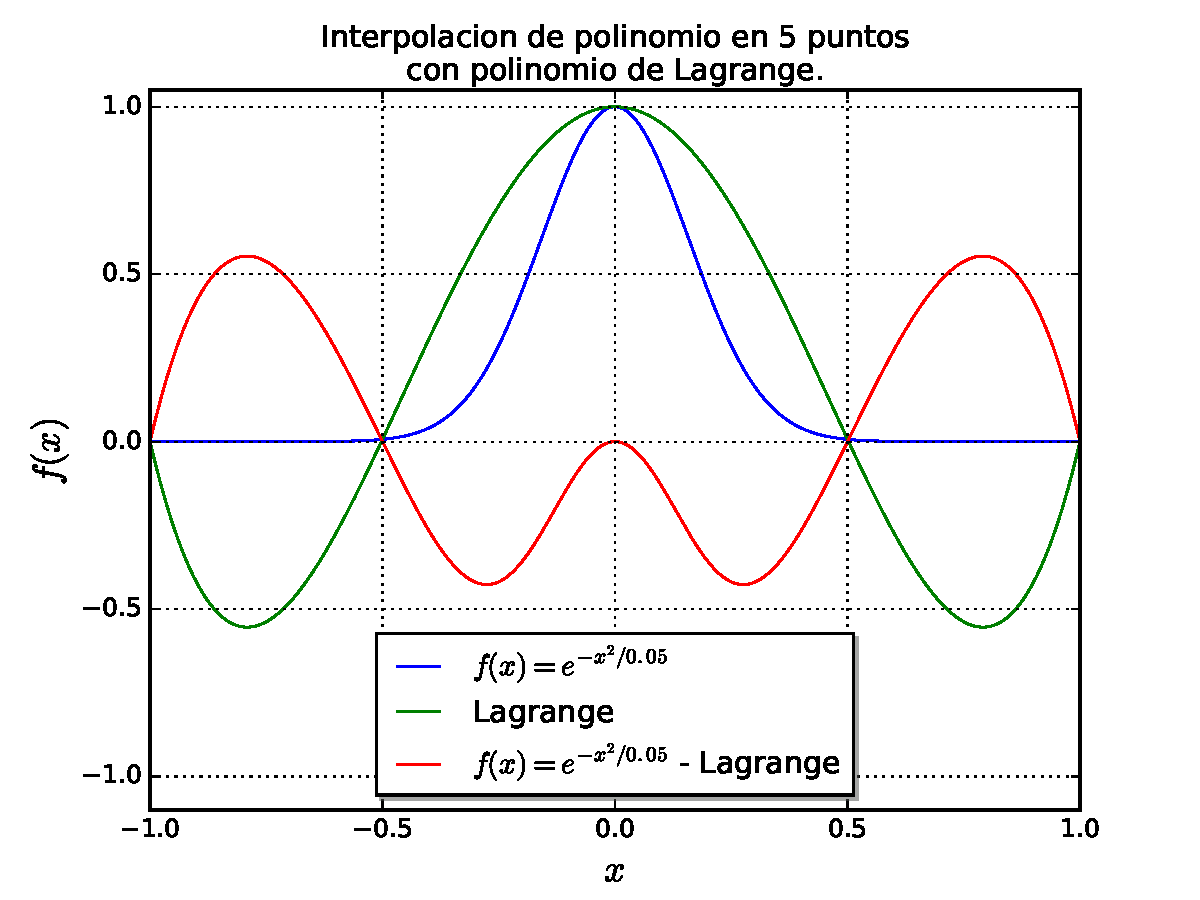
\includegraphics[width=9cm, height=7cm]{img/lagrange5.pdf}
  \caption{Interpolaci\'on con Lagrange para un intervalo\\ $[-1,1]$ equiespaciado con 5 puntos.}
\end{subfigure}%
\begin{subfigure}{.5\textwidth}
  \centering
  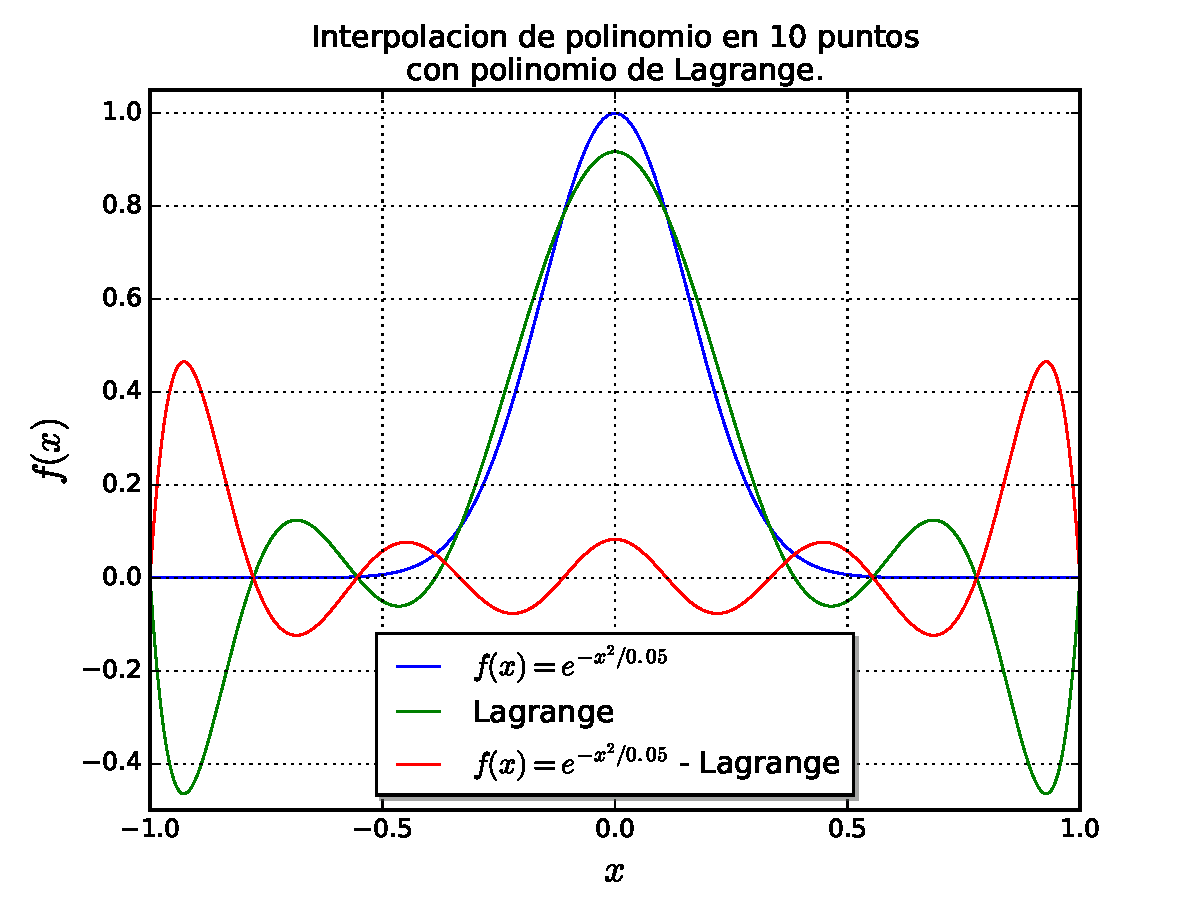
\includegraphics[width=9cm, height=7cm]{img/lagrange10.pdf}
  \caption{Interpolaci\'on con Lagrange para un intervalo\\ $[-1,1]$ equiespaciado con 10 puntos.}
\end{subfigure}
\begin{subfigure}{.5\textwidth}
  \centering
  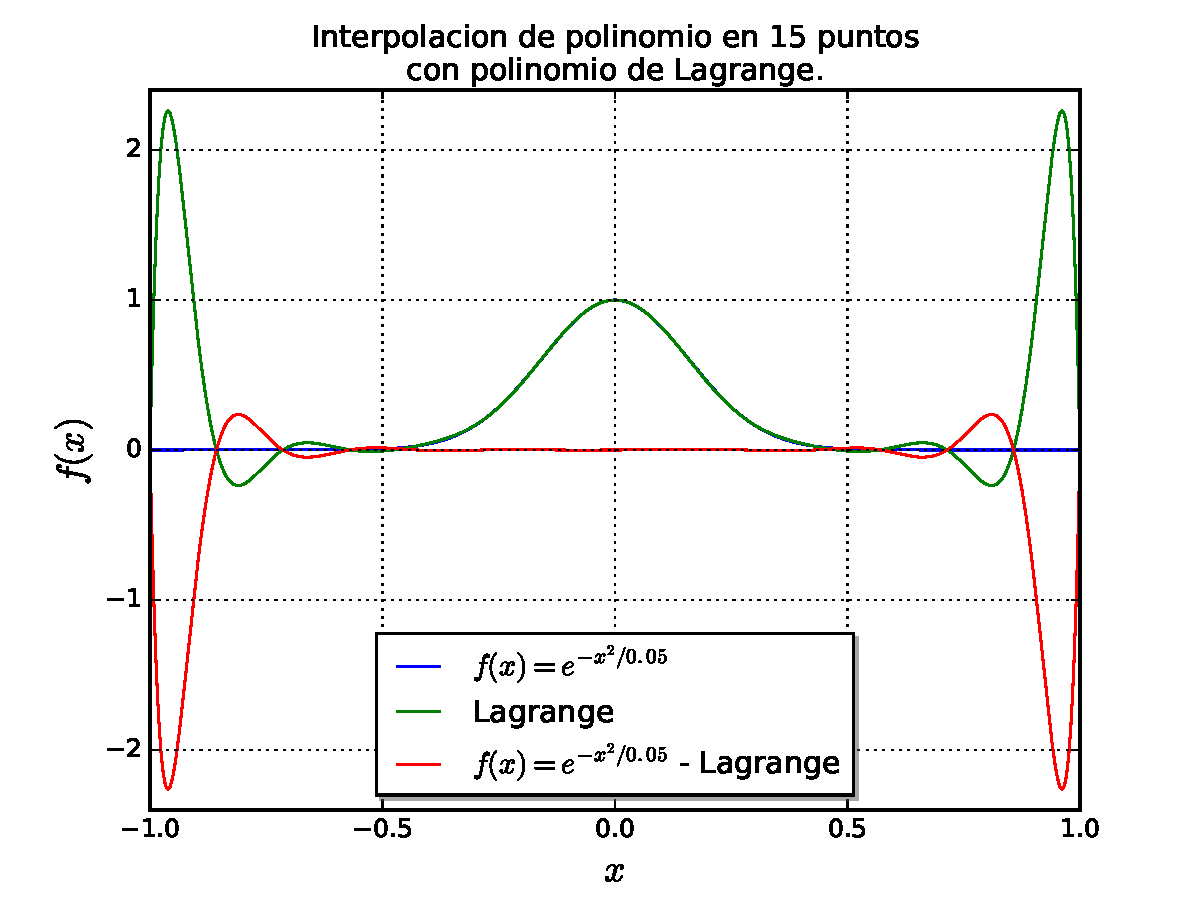
\includegraphics[width=9cm, height=7cm]{img/lagrange15.pdf}
  \caption{Interpolaci\'on con Lagrange para un intervalo\\ $[-1,1]$ equiespaciado con 15 puntos.}
\end{subfigure}%
\begin{subfigure}{.5\textwidth}
  \centering
  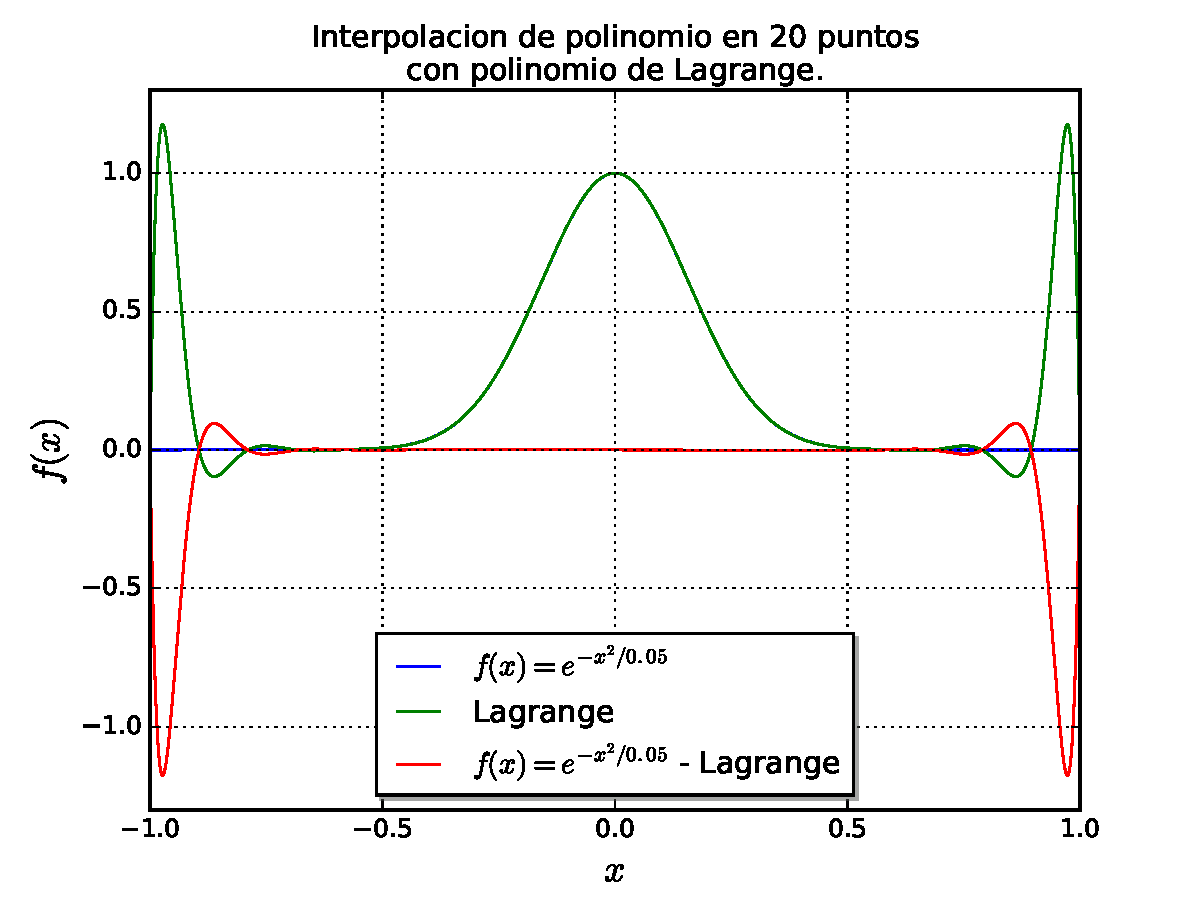
\includegraphics[width=9cm, height=7cm]{img/lagrange20.pdf}
  \caption{Interpolaci\'on con Lagrange para un intervalo\\ $[-1,1]$ equiespaciado con 20 puntos.}
\end{subfigure}
\caption{Distintas interpolaciones utilizando polinomios de Lagrange.}
\end{figure}

\begin{figure}[!hbpt]
\centering
\begin{subfigure}{.5\textwidth}
  \centering
  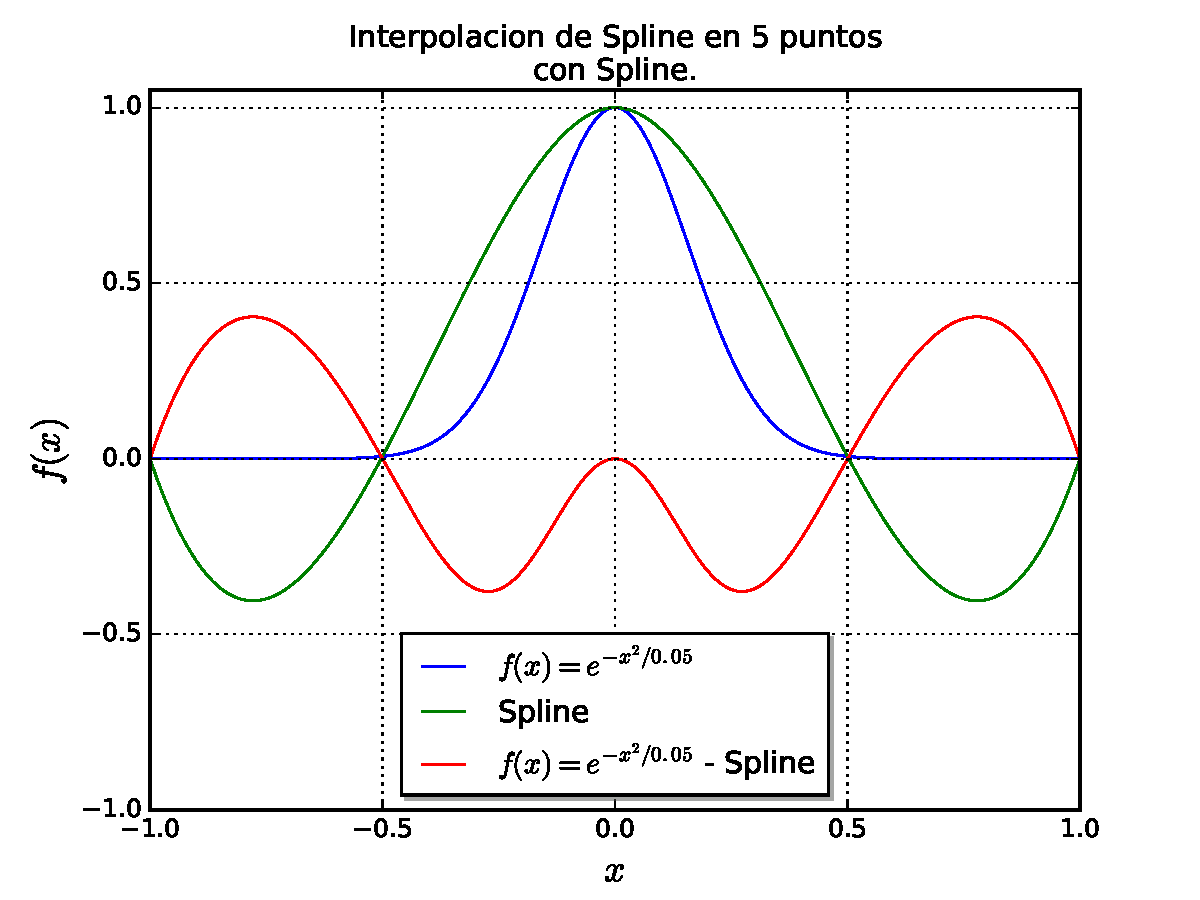
\includegraphics[width=9cm, height=7cm]{img/spline5.pdf}
  \caption{Interpolaci\'on con Spline para un intervalo\\ $[-1,1]$ equiespaciado con 5 puntos.}
\end{subfigure}%
\begin{subfigure}{.5\textwidth}
  \centering
  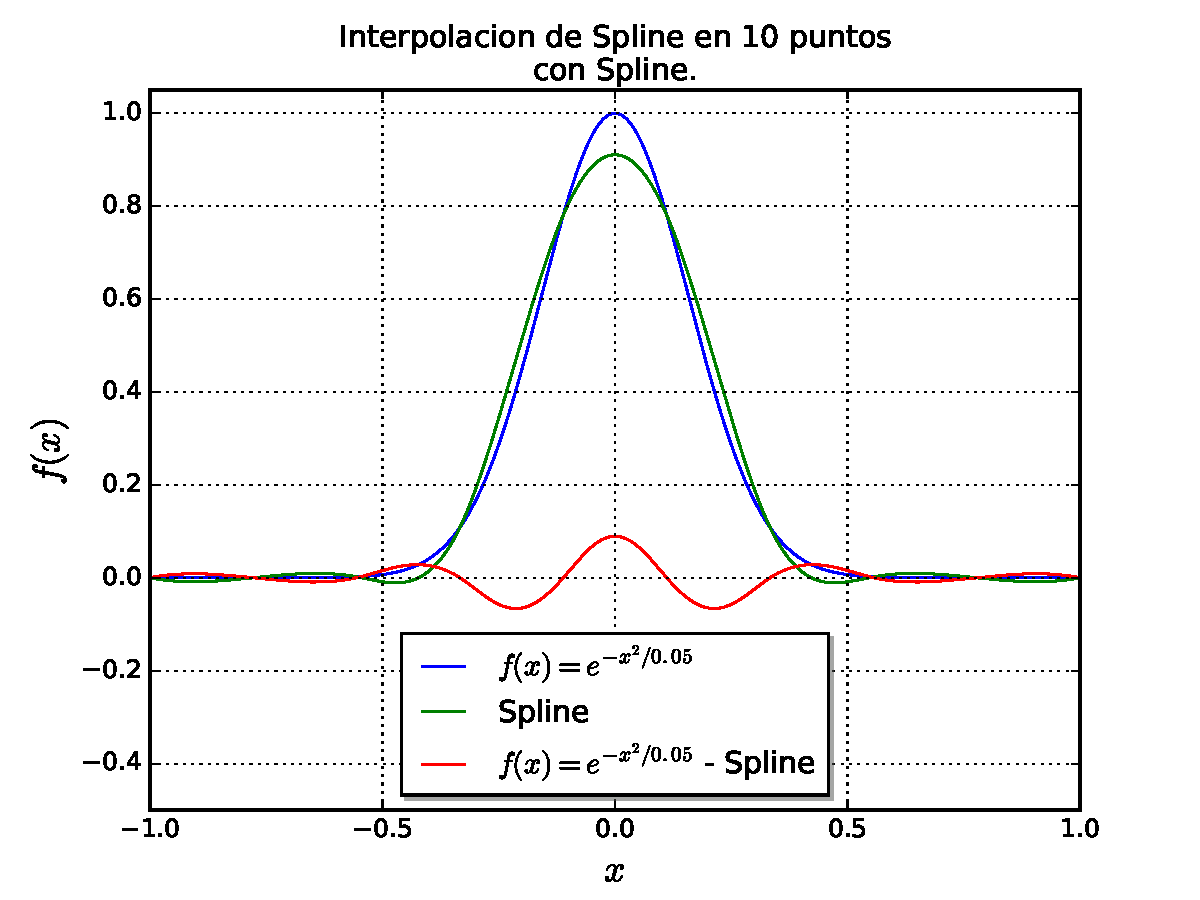
\includegraphics[width=9cm, height=7cm]{img/spline10.pdf}
  \caption{Interpolaci\'on con Spline para un intervalo\\ $[-1,1]$ equiespaciado con 10 puntos.}
\end{subfigure}
\begin{subfigure}{.5\textwidth}
  \centering
  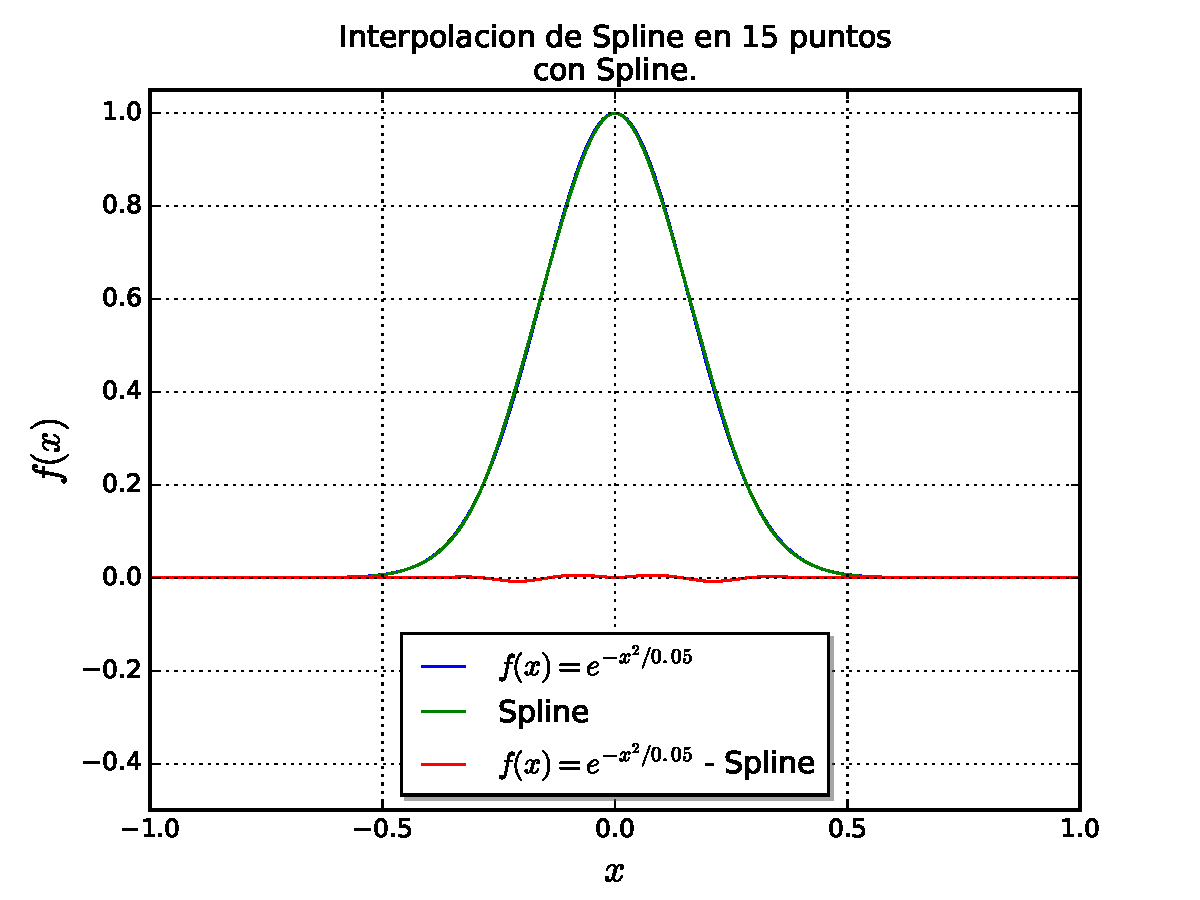
\includegraphics[width=9cm, height=7cm]{img/spline15.pdf}
  \caption{Interpolaci\'on con Spline para un intervalo\\ $[-1,1]$ equiespaciado con 15 puntos.}
\end{subfigure}%
\begin{subfigure}{.5\textwidth}
  \centering
  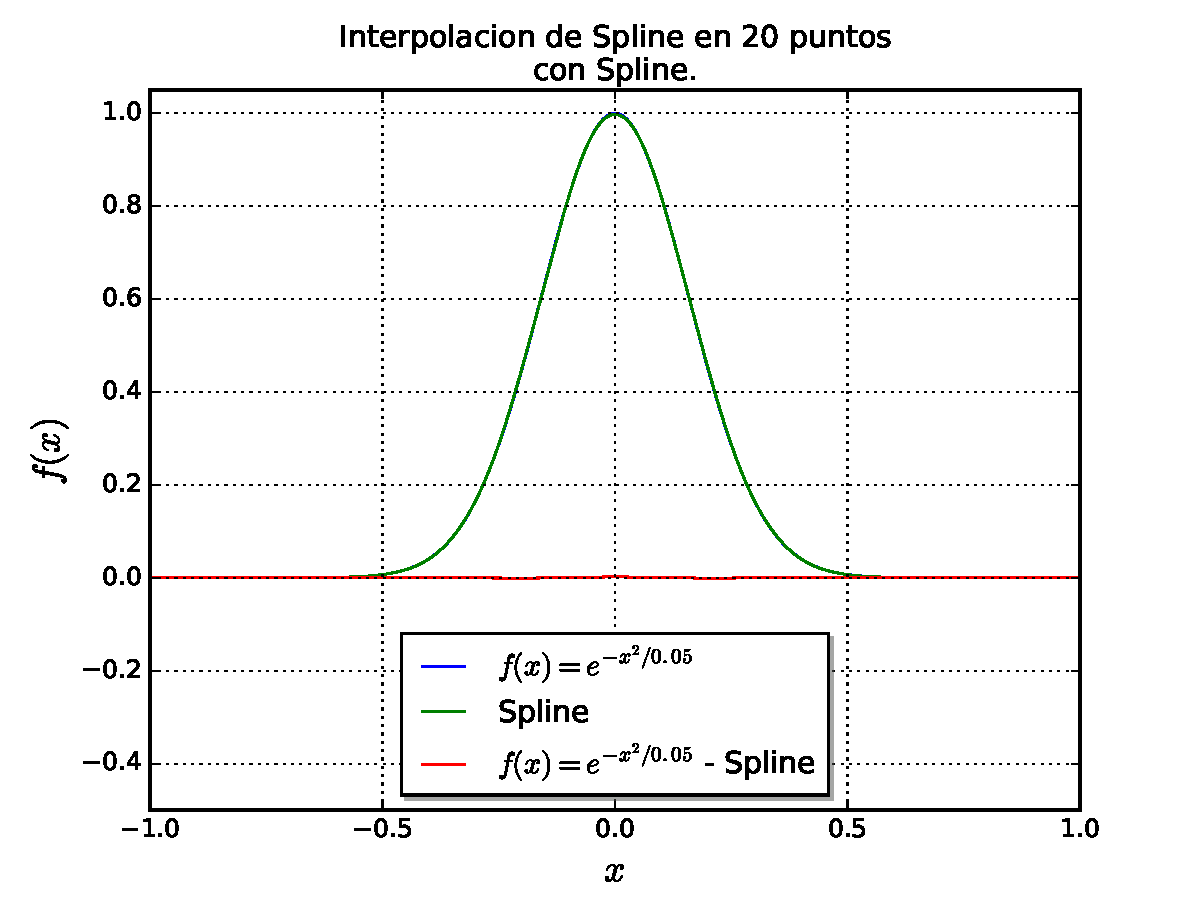
\includegraphics[width=9cm, height=7cm]{img/spline20.pdf}
  \caption{Interpolaci\'on con Spline para un intervalo\\ $[-1,1]$ equiespaciado con 20 puntos.}
\end{subfigure}
\caption{Distintas interpolaciones utilizando Spline.}
\end{figure}

\fig{lagrange_spl_diff.pdf}{18cm}{13cm}{Diferencia entre la funci\'on original y las aproximaciones de Lagrnge y Spline para 50 puntos en el intervalo $[-1, 1]$.}
\fig{fixed_galaxy.pdf}{18cm}{13cm}{Imagen arreglada de la galaxia.}

\newpage

\section{Conclusiones}
Se concluye que una interpolaci\'on con Spline c\'ubico es una mejor aproximaci\'on a mayor cantidad de puntos que una interpolaci\'on con un polinomio de Lagrange, o si es de inter\'es analizar los extremos de la funci\'on a interpolar ya que, a diferencia de \'esta, Spline no presenta el Fen\'omeno de Runge.

Se concluye que la interpolaci\'on es una herramienta \'util en el an\'alisis de im\'agenes, en particular si se busca reparar una imagen da\~nada.

\end{document}
